\documentclass{kdo}
\usepackage{nth}
\usepackage{url}
\usepackage{chants}
\usepackage{multicol}

\renewenvironment{chanttext}{}{}
\renewcommand{\chanttitle}[1]{\pagebreak[3]\section{#1}}

\renewcommand\largebell\relax
\renewcommand\smallbell\relax
\renewcommand\bok\relax
\renewcommand\clank\relax
\renewcommand\muffle\relax
\renewcommand\smallBellRolldown\relax
\renewcommand\bat[1]\relax
\renewcommand\doshidependent[1]{#1}

\begin{document}
\frontmatter
\begin{titlepage}
  \Huge\bf
Kannon Do Chants
\end{titlepage}

\cleardoublepage\thispagestyle{empty}\null\cleardoublepage\frontmatter

\begin{titlepage}
  \Huge\bf
Kannon Do Chants
\end{titlepage}

\begin{colophon}
Kannon Do Chants, Second Printing

\bigskip

\copyright\ 2015, Kannon Do Zen Meditation Center\\
1972 Rock Street, Mountain View, CA 94304\\
www.kannondo.org

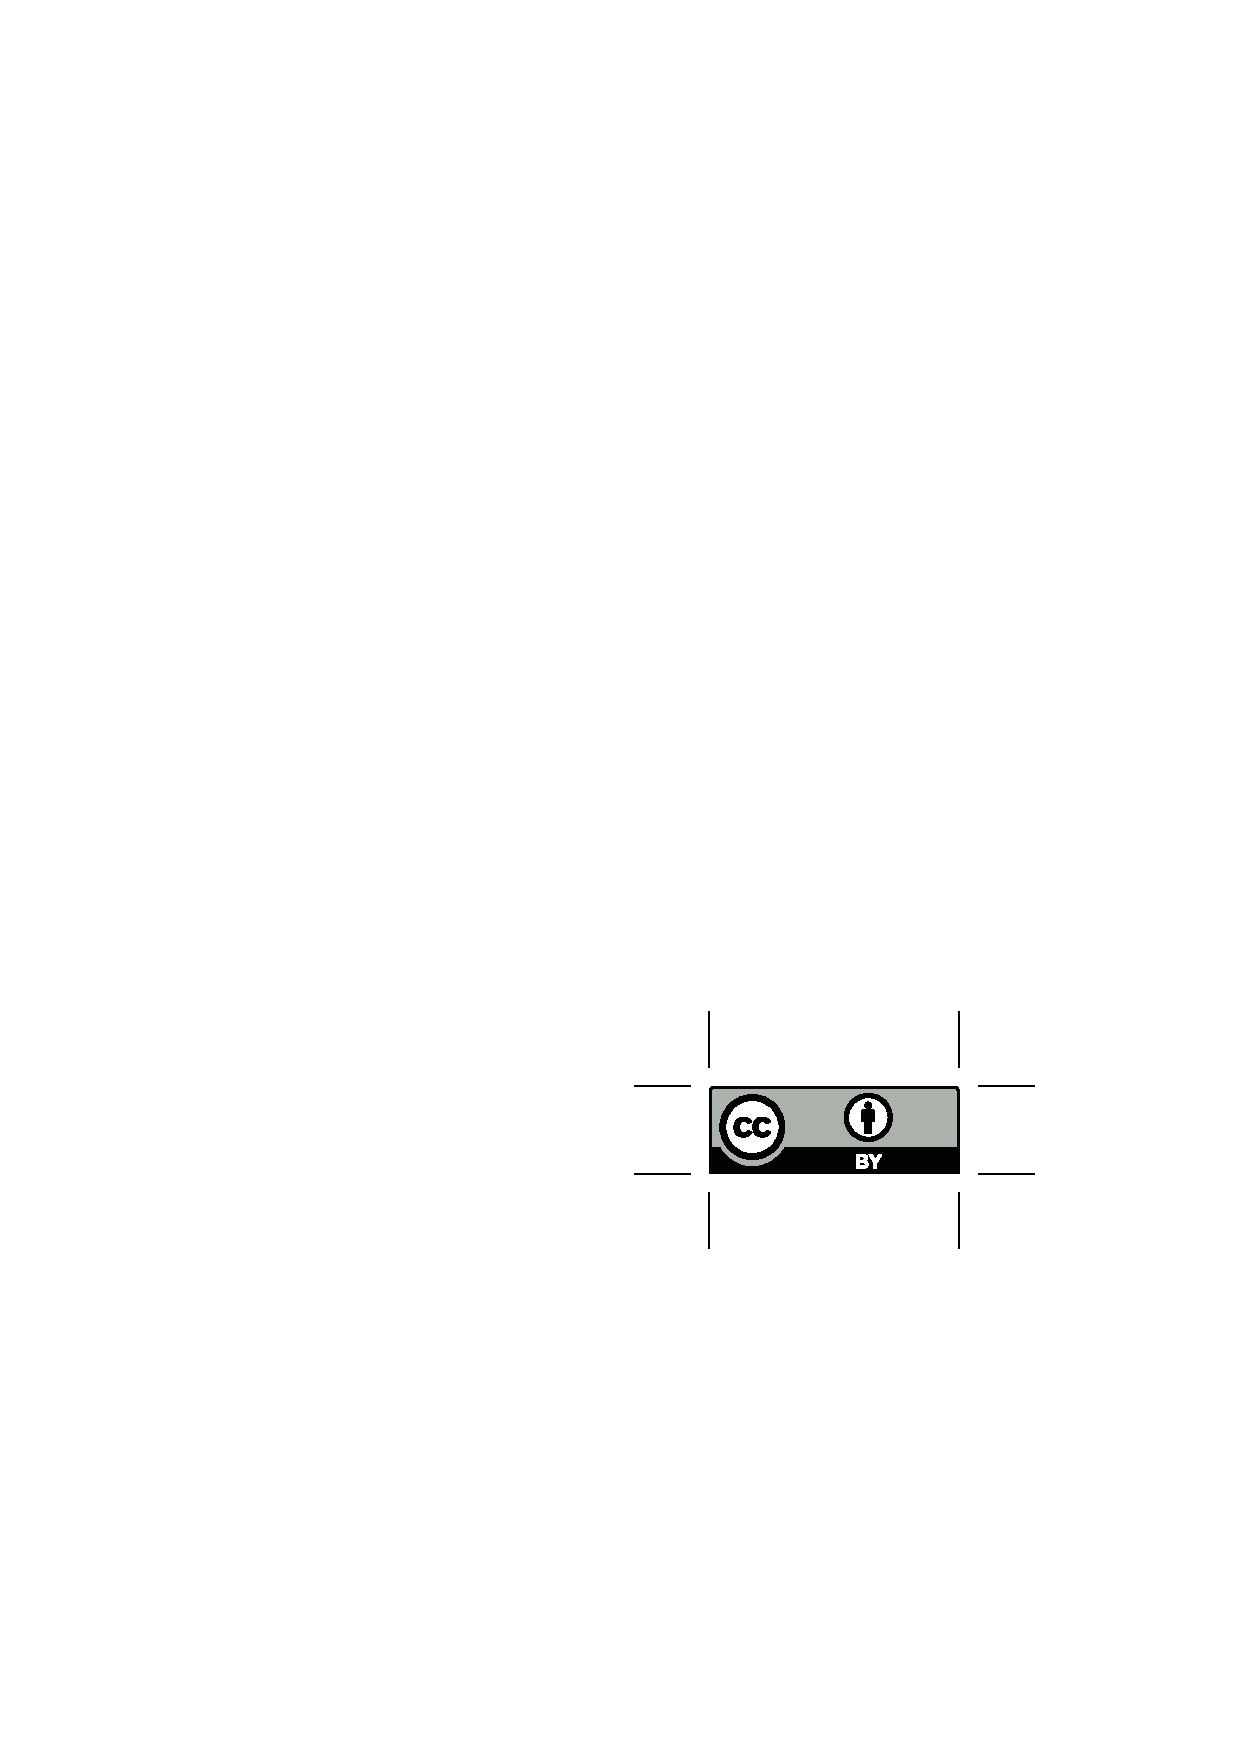
\includegraphics{by}

This work is licensed under the Creative Commons Attribution 4.0 International
License. To view a copy of this license, visit\\
\url{http://creativecommons.org/licenses/by/4.0/}.

\bigskip

This book is set in 14\,pt.\ Fira Sans with \LaTeX\ and hand bound at Kannon Do.
\end{colophon}

\begin{dedication}
One thing flows into another\\
and cannot be grasped.\\
Before the rain stops, we hear a bird.

---Shunryu Suzuki
\end{dedication}

\cleardoublepage

\tableofcontents

\mainmatter
\fontsize{14pt}{16pt plus 2pt}

\part{Wednesday Night}
\chapter{Wednesday Night}
\thumb{Wednesday Night}
\heartOfGreatPerfectWisdomSutra
\allBuddhas
\sutraOpeningVerse
\pagebreak
\fourVows

\part{First and Third Saturdays}
\chapter{First and Third Saturdays}
\thumb{\nth{1} \& \nth{3} Saturday}
\paliRefuges
\makaHannyaHaramittaShingyo
\enmeiJukkuKannonGyo
\songOfTheJewelMirrorSamadhi
\ancestorsShort
\femaleAncestors
\pagebreak
\jiHoSan

\part{Second and Fifth Saturdays}
\chapter{Second and Fifth Saturdays}
\thumb{\nth{2} \& \nth{5} Saturday}
\paliRefuges
\makaHannyaHaramittaShingyo
\shosaimyoKichijoDharani
\harmonyOfDifferenceAndEquality
\ancestorsLong
\jiHoSan

\part{Fourth Saturday}
\chapter{Fourth Saturday}
\thumb{\nth{4} Saturday}
\paliRefuges
\makaHannyaHaramittaShingyo
\shosaimyoKichijoDharani
\lovingKindnessMeditation
\enmeiJukkuKannonGyo
\jiHoSan

\part{Other Chants}
\chapter{Other Chants}
% TODO:
% - Universally recommended instructions for Zazen
% - Daihi Shin Dahrani
% - Robe Chant
\end{document}
